\documentclass[]{article}
\usepackage{lmodern}
\usepackage{amssymb,amsmath}
\usepackage{ifxetex,ifluatex}
\usepackage{fixltx2e} % provides \textsubscript
\ifnum 0\ifxetex 1\fi\ifluatex 1\fi=0 % if pdftex
  \usepackage[T1]{fontenc}
  \usepackage[utf8]{inputenc}
\else % if luatex or xelatex
  \ifxetex
    \usepackage{mathspec}
  \else
    \usepackage{fontspec}
  \fi
  \defaultfontfeatures{Ligatures=TeX,Scale=MatchLowercase}
\fi
% use upquote if available, for straight quotes in verbatim environments
\IfFileExists{upquote.sty}{\usepackage{upquote}}{}
% use microtype if available
\IfFileExists{microtype.sty}{%
\usepackage{microtype}
\UseMicrotypeSet[protrusion]{basicmath} % disable protrusion for tt fonts
}{}
\usepackage[margin=0.6in]{geometry}
\usepackage{hyperref}
\hypersetup{unicode=true,
            pdftitle={Two Lines, Different Slopes (Crocodiles Continued)},
            pdfborder={0 0 0},
            breaklinks=true}
\urlstyle{same}  % don't use monospace font for urls
\usepackage{color}
\usepackage{fancyvrb}
\newcommand{\VerbBar}{|}
\newcommand{\VERB}{\Verb[commandchars=\\\{\}]}
\DefineVerbatimEnvironment{Highlighting}{Verbatim}{commandchars=\\\{\}}
% Add ',fontsize=\small' for more characters per line
\usepackage{framed}
\definecolor{shadecolor}{RGB}{248,248,248}
\newenvironment{Shaded}{\begin{snugshade}}{\end{snugshade}}
\newcommand{\KeywordTok}[1]{\textcolor[rgb]{0.13,0.29,0.53}{\textbf{#1}}}
\newcommand{\DataTypeTok}[1]{\textcolor[rgb]{0.13,0.29,0.53}{#1}}
\newcommand{\DecValTok}[1]{\textcolor[rgb]{0.00,0.00,0.81}{#1}}
\newcommand{\BaseNTok}[1]{\textcolor[rgb]{0.00,0.00,0.81}{#1}}
\newcommand{\FloatTok}[1]{\textcolor[rgb]{0.00,0.00,0.81}{#1}}
\newcommand{\ConstantTok}[1]{\textcolor[rgb]{0.00,0.00,0.00}{#1}}
\newcommand{\CharTok}[1]{\textcolor[rgb]{0.31,0.60,0.02}{#1}}
\newcommand{\SpecialCharTok}[1]{\textcolor[rgb]{0.00,0.00,0.00}{#1}}
\newcommand{\StringTok}[1]{\textcolor[rgb]{0.31,0.60,0.02}{#1}}
\newcommand{\VerbatimStringTok}[1]{\textcolor[rgb]{0.31,0.60,0.02}{#1}}
\newcommand{\SpecialStringTok}[1]{\textcolor[rgb]{0.31,0.60,0.02}{#1}}
\newcommand{\ImportTok}[1]{#1}
\newcommand{\CommentTok}[1]{\textcolor[rgb]{0.56,0.35,0.01}{\textit{#1}}}
\newcommand{\DocumentationTok}[1]{\textcolor[rgb]{0.56,0.35,0.01}{\textbf{\textit{#1}}}}
\newcommand{\AnnotationTok}[1]{\textcolor[rgb]{0.56,0.35,0.01}{\textbf{\textit{#1}}}}
\newcommand{\CommentVarTok}[1]{\textcolor[rgb]{0.56,0.35,0.01}{\textbf{\textit{#1}}}}
\newcommand{\OtherTok}[1]{\textcolor[rgb]{0.56,0.35,0.01}{#1}}
\newcommand{\FunctionTok}[1]{\textcolor[rgb]{0.00,0.00,0.00}{#1}}
\newcommand{\VariableTok}[1]{\textcolor[rgb]{0.00,0.00,0.00}{#1}}
\newcommand{\ControlFlowTok}[1]{\textcolor[rgb]{0.13,0.29,0.53}{\textbf{#1}}}
\newcommand{\OperatorTok}[1]{\textcolor[rgb]{0.81,0.36,0.00}{\textbf{#1}}}
\newcommand{\BuiltInTok}[1]{#1}
\newcommand{\ExtensionTok}[1]{#1}
\newcommand{\PreprocessorTok}[1]{\textcolor[rgb]{0.56,0.35,0.01}{\textit{#1}}}
\newcommand{\AttributeTok}[1]{\textcolor[rgb]{0.77,0.63,0.00}{#1}}
\newcommand{\RegionMarkerTok}[1]{#1}
\newcommand{\InformationTok}[1]{\textcolor[rgb]{0.56,0.35,0.01}{\textbf{\textit{#1}}}}
\newcommand{\WarningTok}[1]{\textcolor[rgb]{0.56,0.35,0.01}{\textbf{\textit{#1}}}}
\newcommand{\AlertTok}[1]{\textcolor[rgb]{0.94,0.16,0.16}{#1}}
\newcommand{\ErrorTok}[1]{\textcolor[rgb]{0.64,0.00,0.00}{\textbf{#1}}}
\newcommand{\NormalTok}[1]{#1}
\usepackage{graphicx,grffile}
\makeatletter
\def\maxwidth{\ifdim\Gin@nat@width>\linewidth\linewidth\else\Gin@nat@width\fi}
\def\maxheight{\ifdim\Gin@nat@height>\textheight\textheight\else\Gin@nat@height\fi}
\makeatother
% Scale images if necessary, so that they will not overflow the page
% margins by default, and it is still possible to overwrite the defaults
% using explicit options in \includegraphics[width, height, ...]{}
\setkeys{Gin}{width=\maxwidth,height=\maxheight,keepaspectratio}
\IfFileExists{parskip.sty}{%
\usepackage{parskip}
}{% else
\setlength{\parindent}{0pt}
\setlength{\parskip}{6pt plus 2pt minus 1pt}
}
\setlength{\emergencystretch}{3em}  % prevent overfull lines
\providecommand{\tightlist}{%
  \setlength{\itemsep}{0pt}\setlength{\parskip}{0pt}}
\setcounter{secnumdepth}{0}
% Redefines (sub)paragraphs to behave more like sections
\ifx\paragraph\undefined\else
\let\oldparagraph\paragraph
\renewcommand{\paragraph}[1]{\oldparagraph{#1}\mbox{}}
\fi
\ifx\subparagraph\undefined\else
\let\oldsubparagraph\subparagraph
\renewcommand{\subparagraph}[1]{\oldsubparagraph{#1}\mbox{}}
\fi

%%% Use protect on footnotes to avoid problems with footnotes in titles
\let\rmarkdownfootnote\footnote%
\def\footnote{\protect\rmarkdownfootnote}

%%% Change title format to be more compact
\usepackage{titling}

% Create subtitle command for use in maketitle
\newcommand{\subtitle}[1]{
  \posttitle{
    \begin{center}\large#1\end{center}
    }
}

\setlength{\droptitle}{-2em}

  \title{Two Lines, Different Slopes (Crocodiles Continued)}
    \pretitle{\vspace{\droptitle}\centering\huge}
  \posttitle{\par}
    \author{}
    \preauthor{}\postauthor{}
    \date{}
    \predate{}\postdate{}
  
\usepackage{soul}
\usepackage{booktabs}

\begin{document}
\maketitle

We have measurements of the head length (cm) and total body length (cm)
of 32 crocodiles of two different species:

\begin{Shaded}
\begin{Highlighting}[]
\KeywordTok{head}\NormalTok{(crocs, }\DecValTok{3}\NormalTok{)}
\end{Highlighting}
\end{Shaded}

\begin{verbatim}
##   Body Head    Species
## 1  338 52.0     Indian
## 2  333 48.0 Australian
## 3  202 38.3     Indian
\end{verbatim}

\textbf{2 lines by filtering to create separate data sets}

\begin{Shaded}
\begin{Highlighting}[]
\NormalTok{aus_crocs <-}\StringTok{ }\NormalTok{crocs }\OperatorTok\StringTok{ }\KeywordTok{filter}\NormalTok{(Species }\OperatorTok{==}\StringTok{ "Australian"}\NormalTok{)}
\NormalTok{aus_fit <-}\StringTok{ }\KeywordTok{lm}\NormalTok{(Head }\OperatorTok{~}\StringTok{ }\NormalTok{Body, }\DataTypeTok{data =}\NormalTok{ aus_crocs)}
\KeywordTok{summary}\NormalTok{(aus_fit)}
\end{Highlighting}
\end{Shaded}

\begin{verbatim}
## 
## Call:
## lm(formula = Head ~ Body, data = aus_crocs)
## 
## Residuals:
##     Min      1Q  Median      3Q     Max 
## -2.3529 -0.9968  0.0824  0.7419  2.7973 
## 
## Coefficients:
##             Estimate Std. Error t value Pr(>|t|)    
## (Intercept) 3.463022   1.523732   2.273   0.0407 *  
## Body        0.125344   0.004819  26.010 1.35e-12 ***
## ---
## Signif. codes:  0 '***' 0.001 '**' 0.01 '*' 0.05 '.' 0.1 ' ' 1
## 
## Residual standard error: 1.504 on 13 degrees of freedom
## Multiple R-squared:  0.9811, Adjusted R-squared:  0.9797 
## F-statistic: 676.5 on 1 and 13 DF,  p-value: 1.35e-12
\end{verbatim}

\begin{Shaded}
\begin{Highlighting}[]
\NormalTok{ind_crocs <-}\StringTok{ }\NormalTok{crocs }\OperatorTok\StringTok{ }\KeywordTok{filter}\NormalTok{(Species }\OperatorTok{==}\StringTok{ "Indian"}\NormalTok{)}
\NormalTok{ind_fit <-}\StringTok{ }\KeywordTok{lm}\NormalTok{(Head }\OperatorTok{~}\StringTok{ }\NormalTok{Body, }\DataTypeTok{data =}\NormalTok{ ind_crocs)}
\KeywordTok{summary}\NormalTok{(ind_fit)}
\end{Highlighting}
\end{Shaded}

\begin{verbatim}
## 
## Call:
## lm(formula = Head ~ Body, data = ind_crocs)
## 
## Residuals:
##     Min      1Q  Median      3Q     Max 
## -4.5756 -1.6627 -0.0904  1.2208  4.6261 
## 
## Coefficients:
##              Estimate Std. Error t value Pr(>|t|)    
## (Intercept) 10.538438   1.861787    5.66 4.53e-05 ***
## Body         0.131304   0.005791   22.68 5.08e-13 ***
## ---
## Signif. codes:  0 '***' 0.001 '**' 0.01 '*' 0.05 '.' 0.1 ' ' 1
## 
## Residual standard error: 2.503 on 15 degrees of freedom
## Multiple R-squared:  0.9717, Adjusted R-squared:  0.9698 
## F-statistic: 514.2 on 1 and 15 DF,  p-value: 5.08e-13
\end{verbatim}

\newpage

\subsubsection{1 model, 2 lines (different
slopes)}\label{model-2-lines-different-slopes}

\begin{itemize}
\tightlist
\item
  Last class we used this code to fit 2 lines with the same slope:
\end{itemize}

\begin{Shaded}
\begin{Highlighting}[]
\NormalTok{parallel_lines_fit <-}\StringTok{ }\KeywordTok{lm}\NormalTok{(Head }\OperatorTok{~}\StringTok{ }\NormalTok{Body }\OperatorTok{+}\StringTok{ }\NormalTok{Species, }\DataTypeTok{data =}\NormalTok{ crocs)}
\end{Highlighting}
\end{Shaded}

\begin{itemize}
\tightlist
\item
  To allow for different slopes, use \texttt{*} instead of \texttt{+}
\end{itemize}

\begin{Shaded}
\begin{Highlighting}[]
\NormalTok{two_lines_fit <-}\StringTok{ }\KeywordTok{lm}\NormalTok{(Head }\OperatorTok{~}\StringTok{ }\NormalTok{Body }\OperatorTok{*}\StringTok{ }\NormalTok{Species, }\DataTypeTok{data =}\NormalTok{ crocs)}
\KeywordTok{summary}\NormalTok{(two_lines_fit)}
\end{Highlighting}
\end{Shaded}

\begin{verbatim}
## 
## Call:
## lm(formula = Head ~ Body * Species, data = crocs)
## 
## Residuals:
##     Min      1Q  Median      3Q     Max 
## -4.5756 -1.3294 -0.0040  0.9646  4.6261 
## 
## Coefficients:
##                    Estimate Std. Error t value Pr(>|t|)    
## (Intercept)        3.463022   2.126572   1.628   0.1146    
## Body               0.125344   0.006726  18.637   <2e-16 ***
## SpeciesIndian      7.075415   2.638253   2.682   0.0121 *  
## Body:SpeciesIndian 0.005959   0.008296   0.718   0.4785    
## ---
## Signif. codes:  0 '***' 0.001 '**' 0.01 '*' 0.05 '.' 0.1 ' ' 1
## 
## Residual standard error: 2.099 on 28 degrees of freedom
## Multiple R-squared:  0.9775, Adjusted R-squared:  0.975 
## F-statistic: 404.6 on 3 and 28 DF,  p-value: < 2.2e-16
\end{verbatim}

\begin{Shaded}
\begin{Highlighting}[]
\NormalTok{crocs <-}\StringTok{ }\NormalTok{crocs }\OperatorTok
\StringTok{  }\KeywordTok{mutate}\NormalTok{(}
    \DataTypeTok{fitted =} \KeywordTok{predict}\NormalTok{(two_lines_fit)}
\NormalTok{  )}

\KeywordTok{ggplot}\NormalTok{(}\DataTypeTok{data =}\NormalTok{ crocs) }\OperatorTok{+}
\StringTok{  }\KeywordTok{geom_point}\NormalTok{(}\DataTypeTok{mapping =} \KeywordTok{aes}\NormalTok{(}\DataTypeTok{x =}\NormalTok{ Body, }\DataTypeTok{y =}\NormalTok{ Head, }\DataTypeTok{color =}\NormalTok{ Species)) }\OperatorTok{+}
\StringTok{  }\KeywordTok{geom_line}\NormalTok{(}\DataTypeTok{mapping =} \KeywordTok{aes}\NormalTok{(}\DataTypeTok{x =}\NormalTok{ Body, }\DataTypeTok{y =}\NormalTok{ fitted, }\DataTypeTok{color =}\NormalTok{ Species))}
\end{Highlighting}
\end{Shaded}

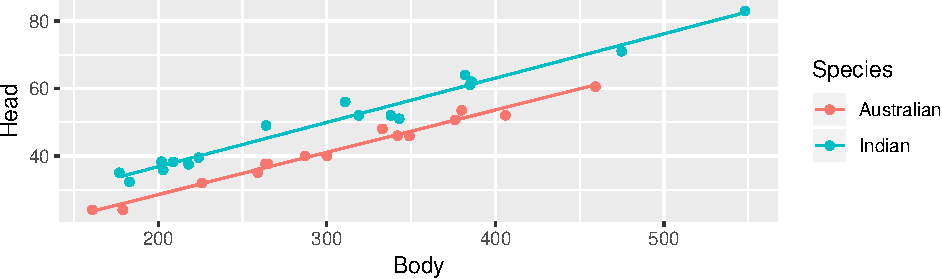
\includegraphics{20190329_two_lines_files/figure-latex/unnamed-chunk-6-1.pdf}

\begin{itemize}
\tightlist
\item
  Recall that \texttt{SpeciesIndian} is an indicator variable defined
  as:
  \[\text{{\tt SpeciesIndian}} = \begin{cases} 1 & \text{ if the species for crocodile $i$ is Indian.} \\
  0 & \text{ otherwise (in this case, the species is Australian)} \end{cases}
  \]
\end{itemize}

\newpage

\paragraph{What is the estimated equation from this
model?}\label{what-is-the-estimated-equation-from-this-model}

\vspace{2.5cm}

\paragraph{What is the estimated equation describing the relationship
between body length and head length, for Australian
crocodiles?}\label{what-is-the-estimated-equation-describing-the-relationship-between-body-length-and-head-length-for-australian-crocodiles}

\vspace{2.5cm}

\paragraph{What is the estimated equation describing the relationship
between body length and head length, for Indian
crocodiles?}\label{what-is-the-estimated-equation-describing-the-relationship-between-body-length-and-head-length-for-indian-crocodiles}

\vspace{2.5cm}

\paragraph{\texorpdfstring{What is the interpretation of
\(\widehat{\beta}_0 = 3.463\)?}{What is the interpretation of \textbackslash{}widehat\{\textbackslash{}beta\}\_0 = 3.463?}}\label{what-is-the-interpretation-of-widehatbeta_0-3.463}

\vspace{2.5cm}

\paragraph{\texorpdfstring{What is the interpretation of
\(\widehat{\beta}_1 = 7.075\)?}{What is the interpretation of \textbackslash{}widehat\{\textbackslash{}beta\}\_1 = 7.075?}}\label{what-is-the-interpretation-of-widehatbeta_1-7.075}

\vspace{2.5cm}

\paragraph{\texorpdfstring{What is the interpretation of
\(\widehat{\beta}_2 = 0.125\)?}{What is the interpretation of \textbackslash{}widehat\{\textbackslash{}beta\}\_2 = 0.125?}}\label{what-is-the-interpretation-of-widehatbeta_2-0.125}

\vspace{2.5cm}

\paragraph{\texorpdfstring{What is the interpretation of
\(\widehat{\beta}_3 = 0.006\)?}{What is the interpretation of \textbackslash{}widehat\{\textbackslash{}beta\}\_3 = 0.006?}}\label{what-is-the-interpretation-of-widehatbeta_3-0.006}

\newpage

\paragraph{\texorpdfstring{Using the output from the summary function,
conduct a test of the claim that the \emph{slope} of the line describing
the relationship between body length and head length in the population
of all Australian crocodiles is the same as the \emph{slope} of the line
describing the relationship between body length and head length in the
population of all Indian
crocodiles.}{Using the output from the summary function, conduct a test of the claim that the slope of the line describing the relationship between body length and head length in the population of all Australian crocodiles is the same as the slope of the line describing the relationship between body length and head length in the population of all Indian crocodiles.}}\label{using-the-output-from-the-summary-function-conduct-a-test-of-the-claim-that-the-slope-of-the-line-describing-the-relationship-between-body-length-and-head-length-in-the-population-of-all-australian-crocodiles-is-the-same-as-the-slope-of-the-line-describing-the-relationship-between-body-length-and-head-length-in-the-population-of-all-indian-crocodiles.}


\end{document}
